\section{Aufbau}
\label{sec:Aufbau}
In \autoref{fig:aufbau} ist der verwendete Versuchaufbau zu finden. Er besteht aus einer optischen Schiene, einem
grünen Justierlaser, einem HeNe-Laserrohr mit eingebauten Brewsterfenstern und zwei hochreflektierenden Spiegeln,
die als optischer Resonator dienen. Die Befestigungen der Spiegel können verschoben werden und die Spiegel können
durch planare oder konkave Spiegel aus gewechselt werden. Die Schiene ist $\SI{2,50}{\meter}$ lang und die konkaven
Spiegel haben einen Krümmungsradius von $r=\SI{1400}{\milli\meter}$. Für die Messung stehen noch ein um $2\pi$
drehbarer Polarisationsfilter, ein Wolframdraht, vier optische Gitter, ein Oszilloskop, zwei Photodioden und ein
Schirm zur Verfügung. Diese Bauteile können alle nach Bedarf auf der Schiene angebracht werden.
\begin{figure}
    \centering
    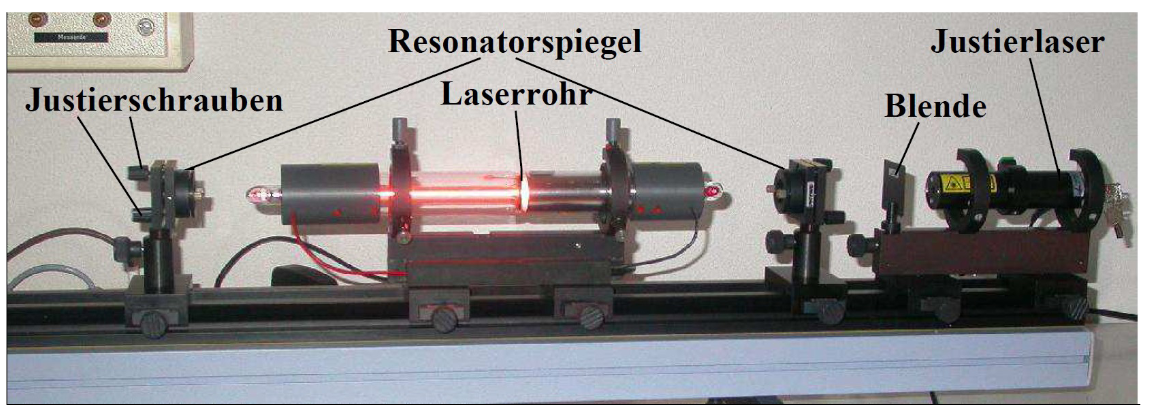
\includegraphics[height=6cm]{content/pics/aufbau.png}
    \caption{Foto des Versuchaufbaus. \cite{V61}}
    \label{fig:aufbau}
\end{figure}

\section{Durchführung}
\label{sec:Durchführung}
Zu aller erst wird der Laser auf seine maximale Leistung justiert. Dazu wird eine Photodiode und ein bereits
eingestellter Justierlaser verwendet. Außerdem gibt es noch Feineinstellungen an den Spiegeln.
Die folgenden Messungen können in beliebiger Reihenfolge durchgeführt werden.

\subsection{Messung der Stabilitätsbedingung}
Die theoretische bestimmte Stabilitätsbedingung wird durch vergrößern des Spiegelabstands und nachjustieren des
Lasers überprüft. Es wird ein konkav-konkav und ein plan-konkav Resonator verwendet. Der Abstand wird so lange
vergrößert bis keine Intensität an der Photodiode messbar ist.

\subsection{Messung der Frequenzbreite}
Während der Stabilitätsmessung bietet es sich an die Schwebungsfequenz zu messen. Dazu wird für unterschiedliche
Spiegelabstände das Signal der Photodiode an einem Oszilloskop zeitlich aufgelöst und die Frequenzen aller
Peaks notiert.

\subsection{Messung der TEM-Moden}
Es wird ein dünner ($d=\SI{0,0005}{\milli\meter}$) Wolframdraht, der als Modenblende fungiert,
zwischen Laserrohr und Spiegel gestellt, so dass die Moden auf einem Schirm zu sehen sind. Anschließend
wird eine Lochblende verwendet, um nur einen geringen Teil des Lichts durch zu lassen und mit einer Photodiode
zu messen. Dies wird für die $TEM_{00}$- und $TEM_{01}$-Mode gemacht.

\subsection{Messung der Polarisation}
Es wird auf der Schiene ein Polarisationsfilter angebracht und mit einer Photodiode die Intensität für volle
$360^{\circ}$ in $10^{\circ}$-Schritten gemessen.

\subsection{Messung der Wellenlänge}
Es werden für vier optische Gitter mit $g=80 \frac{\symup{lines}}{\si{\milli\meter}}$,
$g=100 \frac{\symup{lines}}{\si{\milli\meter}}$, $g=600 \frac{\symup{lines}}{\si{\milli\meter}}$ und
$g=1200 \frac{\symup{lines}}{\si{\milli\meter}}$ auf die Schiene gebaut und die Abstände der n-ten Maxima
zum Maximum nullter Ordnung auf einem optischen Schirm gemessen.